\documentclass[a4paper]{article}

\usepackage[czech]{babel} %https://github.com/michal-h21/biblatex-iso690
\usepackage[
   backend=biber      % if we want unicode 
  ,style=iso-numeric % or iso-numeric for numeric citation method          
  ,babel=other        % to support multiple languages in bibliography
  ,sortlocale=cs_CZ   % locale of main language, it is for sorting
  ,bibencoding=UTF8   % this is necessary only if bibliography file is in different encoding than main document
]{biblatex}

\usepackage[utf8]{inputenc}
\usepackage{fancyhdr}
\usepackage{amsmath}
\usepackage{amssymb}
\usepackage[left=2cm,right=2cm,top=2.5cm,bottom=2.5cm]{geometry}
\usepackage{graphicx}
\usepackage{pdfpages}
\usepackage{url}

\usepackage{siunitx}
\sisetup{locale = DE}  %, separate-uncertainty = true    kdybych chtel +/-

\usepackage{float}
\newfloat{graph}{htbp}{grp}
\floatname{graph}{Graf}
\newfloat{tabulka}{htbp}{tbl}
\floatname{tabulka}{Tabulka}

\renewcommand{\thefootnote}{\roman{footnote}}

\pagestyle{fancy}
\lhead{Praktikum III - (20) Stavba Michelsonova interferometru a ověření jeho funkce}
\rhead{Vladislav Wohlrath}
\author{Vladislav Wohlrath}

\bibliography{source}

\begin{document}

\begin{titlepage}
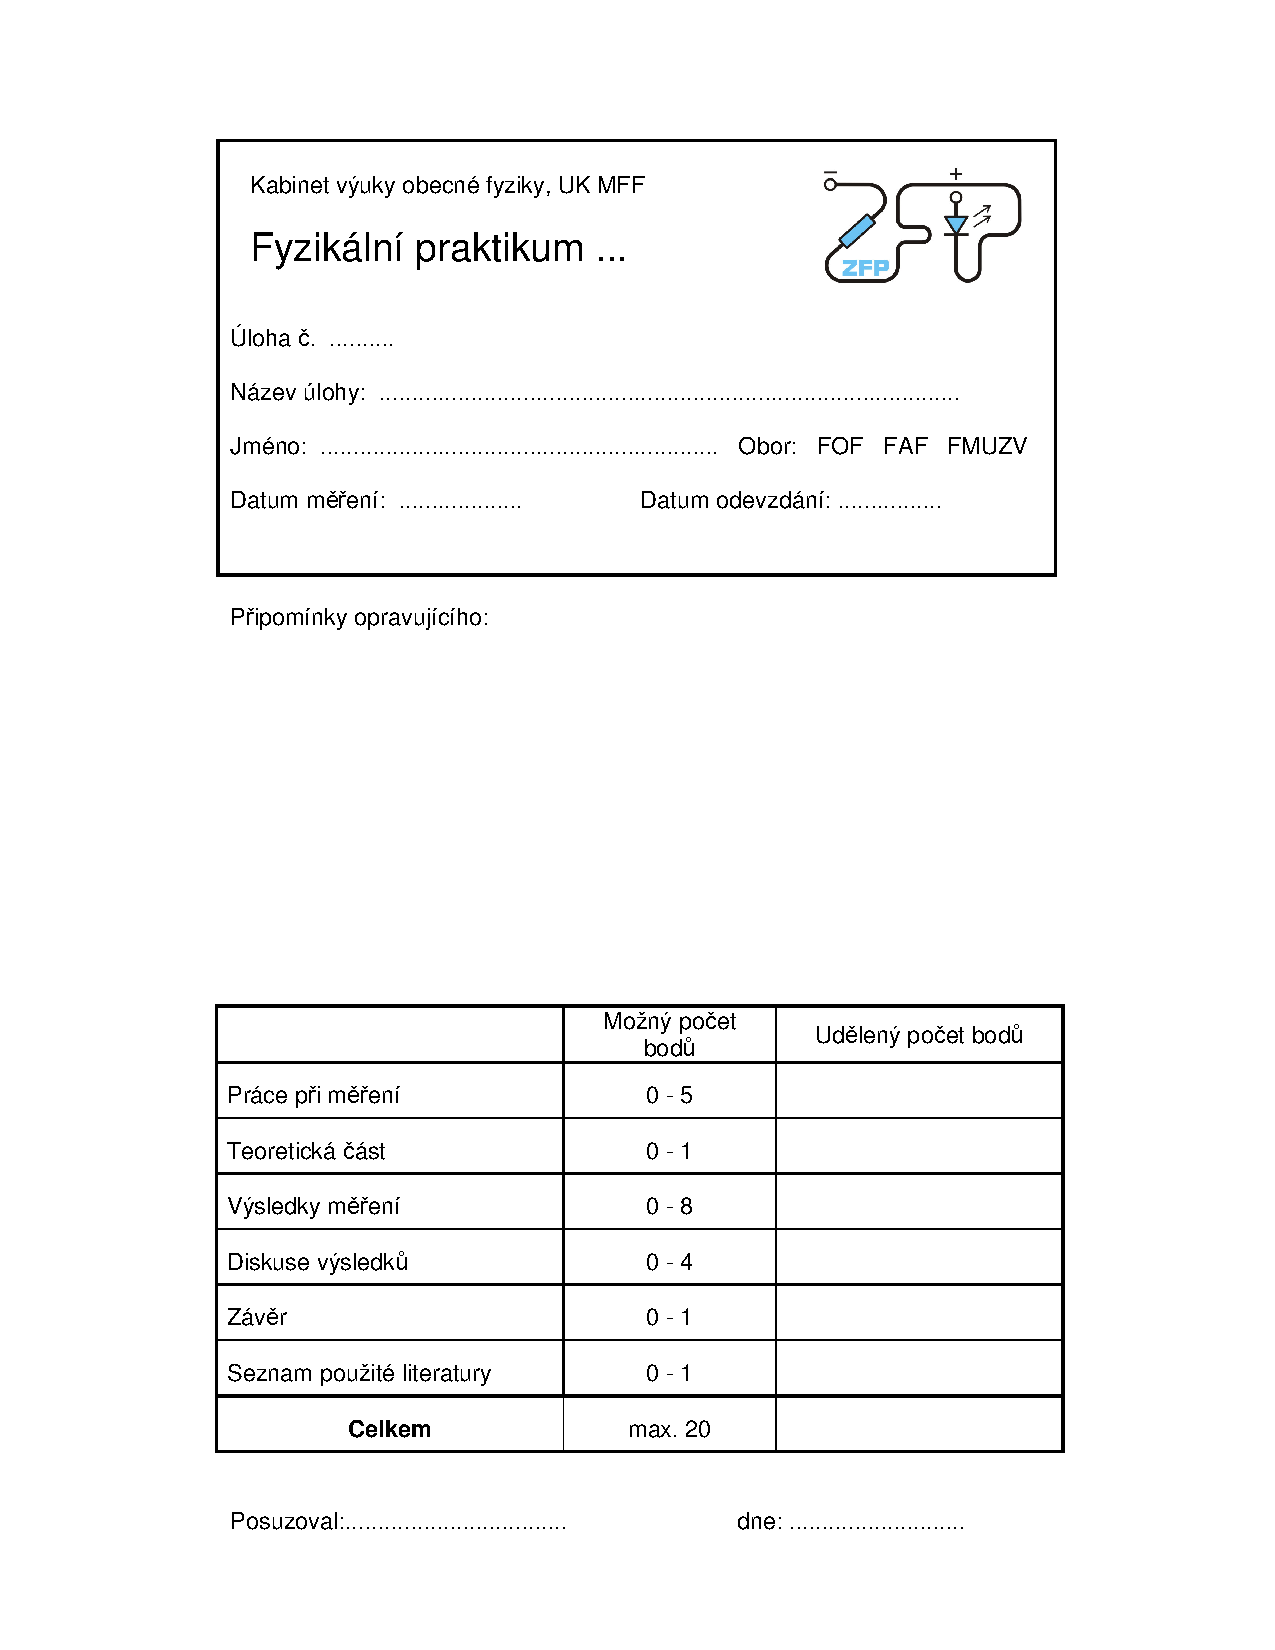
\includepdf[pages={1}]{./graficos/titlelist.pdf}
\end{titlepage}

\section*{Pracovní úkoly}
\begin{enumerate}
\item Změřte divergenci laserového svazku. Průměry svazku změřte na milimetrovém papíru i měřičem profilu svazků a obě metody porovnejte.
\item Sestavte Galileův teleskop. Změřte, kolikrát rozšiřuje průměr svazku, a výsledek porovnejte s výpočtem rozšíření ze známých ohniskových délek čoček.
\item Sestavte Michelsonův interferometr. Vysvětlete princip vzniku interferenčních proužků.
\item Pozorujte, popište a vysvětlete změny v interferenčním obrazci při:
        \begin{enumerate}
        \item naklánění zrcadla Z4,
        \item posunu zrcadla Z3 mikrometrickým šroubem,
        \item vkládání skla do svazku ve čtyřech polohách kolem děliče svazku
        \item ohřátí vzduchu v různých místech průchodu svazku.
        \end{enumerate}

\end{enumerate}

%Teoretická část
\section*{Teoretická část}
Laserový svazek má přibližně gaussovský profil a rozbíhá se.
Rozbíhavost svazku charakterizujeme divergencí\cite{skripta}
\begin{equation} \label{e:div}
d=\frac{D_2-D_1}{s} \,,
\end{equation}
kde $D_1$ je průměr svazku u výstupního otvoru a $D_2$ je průměr svazku ve vzdálenosti $s$.
Minimální dosažitelná divergence $d_m$ lze odhadnout\cite{skripta}
\begin{equation} \label{e:dmin}
d_m=\frac{2\lambda}{D_1} \,,
\end{equation}
kde $\lambda=\SI{632.8}{\nm}$ je vlnová délka použitého světla.


K úpravě šířky svazku použijeme Galileův teleskop. Teleskop je tvořen jednou rozptylnou a jednou spojnou čočkou. V našem případě je ohnisková vzdálenost rozptylné čočky $f_1=\SI{-25}{\mm}$ a spojné čočky $f_2=\SI{200}{\mm}$.
Příčné zvětšení (rozšíření svazku) je pak dáno jejich poměrem 
\begin{equation} \label{e:rozsireni}
\beta=\num{8} \,.
\end{equation}



%Výsledky měření
\section*{Výsledky měření}

%Diskuze výsledků
\section*{Diskuze}
Měření průměru svazku na milimetrovém papíru je neobyčejně nepřesné. Z hodnot průměru svazku je vidět, že jsme při měření na milimetrovém papíru považovali svazek za širší než při měření detektorem. Divergence vyšla pro obě metody shodně a menší než minimální dosažitelná divergence. Poměr změřené divergence a minimální dosažitelné divergence je citlivý na přesnou definici průměru svazku, nestačí jen vždy konzistentně uvažovat stejnou část svazku.
Z tohoto důvodu nepovažujeme výpočet divergence za směroplatný, jelikož ta část paprsku, jejíž průměr jsme měřili, byla určena spíše náhodně a ne v souladu s teorií.

Skutečné zvětšení Galileova teleskopu se shoduje s teoretickou hodnotou v rámci chyby měření, která je však velmi vysoká.

Stavba Michelsonova interferometru proběhla v pořádku.

Všěchny změny v interferenčním obrazci při provádění pracovního úkolu 4 byly ve shodě s teoretickými předpovědmi.

%Závěr
\section*{Závěr}
Změřili jsme divergenci laserového svazku na milimetrovém papíře a měřičem profilu svazků (viz tabulka \ref{t:div}).

Sestavili jsme Galileův teleskop a změřilli jeho příčné zvětšení \num{9(2)}.

Sestavili jsme Michelsonův interferometr. Vysvětlili jsme princip vzniku interferenčních proužků a změny v interferenčním poli při různých změnách podmínek (viz Výsledky).


\printbibliography[title={Seznam použité literatury}]

\end{document}